\documentclass[12pt,oneside]{fithesis}
%\documentclass[12pt,draft,oneside]{fithesis}
\usepackage[utf8]{inputenc}
\usepackage[IL2]{fontenc}
\usepackage[plainpages=false, pdfpagelabels]{hyperref}
\usepackage{paralist}
\usepackage{graphicx}
\usepackage{amsmath}
\usepackage{color}
\usepackage{courier}
\usepackage[czech]{babel}

\usepackage{float}
\floatstyle{ruled}

\thesistitle{Solventnost pojišťovny}
\thesissubtitle{Seminární práce}
\thesisstudent{Marek Bryša}
\thesiswoman{false}
\thesisfaculty{sci}
\thesislang{cz}
\thesisyear{jaro 2012}

\begin{document}
\FrontMatter
\ThesisTitlePage


\MainMatter
\tableofcontents
\chapter{Úvod}
%http://www.skvara.cz/__cw_files/poji%C5%A1t%C4%9Bn%C3%AD/solvencyII/.10/.07/.abe645bf575778fda76cc843d938629e1150540710/SolvencyII.doc
%VZ: ciste pojistne PDF:134
%vl k 67
\chapter{Solvency II}
\chapter{Poměrové ukazatele}
\footnote{Převzato z Růčková: Finanční analýza : metody, ukazatele, využití v praxi, 2.aktualizované vydání, Praha: GRADA Publishing, 2008, ISBN 978-80-247-2481-2, str. 48-50 a Grünwald, Holečková: Finanční analýza a plánování podniku, 1.vydání, Praha: Ekopress, 2007, ISBN 978-80-86929-26-2, str.112-115} Základní metodou analyzování a vykazování solventnosti pojišťovny je série následujících
poměrových ukazatelů vycházející z účetnictví pojišťovny.
\[
	\text{solvency ratio} =\frac{\text{ volný kapitál pojistitele}}{\text{čisté pojistné}}
\]

Solvency ratio neboli ukazatel solventnosti je základním účetním vyjádřením schopnosti
pojišťovny pokrýt své závazky. Volný kapitál jsou prostředky, kterými může pojišťovna
volně disponovat. Čisté pojistné je hodnota pojistného připadající na vrub pojistitele. Hodnota tohoto ukazatele by se měla pohybovat v rozmezí 30 až 50\%.
\[
	\text{retention ratio} =\frac{\text{netto pojistné}}{\text{brutto pojistné}}
\]

Stanovení netto pojistného vychází z teoretického modelu principu ekvivalence, kdy se do
rovnosti pokládají budoucí pojistné závazky a pojistné, které za pokrytí rizik platí pojištění. Brutto neboli hrubé pojistné pak představuje netto pojistné rozšířené o zahrnutí nákladových složek a zisku pojišťovny, které z daného obchodního vztahu vyplívají. Nákladovou složkou rozumíme tzv. správní náklady, které dále členíme na získávací, běžné, inkasní a náklady při výplatě důchodu. Získávací náklady jsou spjaty s mechanismy vynaložené na získání klienta formou pojistné smlouvy ohledně pojistného produktu. Běžné správní nálady jsou vynuceny převážně administrativou a provozními náklady pojištění. Inkasní složka je charakterizována výdaji vzniklými z finančních toků plynoucích z jednotlivých pojistných. Ukazatel je tak vždy menší než-li jedna, neboť netto pojistné dosahuje menších hodnot než-li brutto. Lze jej interpretovat také jakožto ukazatel efektivnosti nákladových složek. Z hlediska likvidity stanovuje, jaká část případných závazků je pokryta běžnými finančními zdroji pojišťovny.
\[
	\text{liquidity ratio} =\frac{\text{likvidní aktiva}}{\text{technické rezervy}}
\]

Poměr likvidních aktiv ku technickým rezervám vyjadřuje, do jaké míry jsou závazky
pojišťovny vyplívající z pojistných vztahů pokryty převážně peněžními prostředky. Tento
ukazatel by se dal připodobnit k indikátoru peněžní likvidity obecné finanční analýzy. Čím
vyšší hodnota liquidity ratio, tím nižší mírou likvidního rizika je pojišťovna vystavena. Na druhou stranu vysoké ukazatele likvidity obecně snižují efektivnost celkového podnikání;
ukazatel technických rezerv = technické rezervy + vlastní kapitál / čisté pojistné
ukazatel technických rezerv (technical coverage ratio ) bývá často modifikován i do podoby
poměru, kdy se v čitateli spolu s průměrným stavem technických rezerv přičítá i průměrný
stav vlastního kapitálu. Hodnota indikátoru by se měla pohybovat v rozmezí 100 až 150\%.
\[
	\text{expenses ratio} =\frac{\text{pořizovací náklady} + \text{režijní náklady}}{\text{brutto pojistné}}
\]

Expenses ratio je nákladovým ukazatelem, a jeho podoba se blíží převrácené hodnotě obratovosti nákladů ve finanční analýze běžných podniků, brutto pojistné lze totiž přirovnat k tržbám podniku. Pořizovací a režijní náklady jsou spjaty se získáním pojištění, údržbou pojistných vztahů a provozem pojišťovny.

\chapter{Příklady}
Následující tabulky byly převzaty z výročních zpráv pojišťoven za rok 2011. Vypočítáme výše uvedené poměrové ukazatele, pokud to dostupná data dovolí. U České pojištovny byl navíc ukazatel technických rezerv rozdělen na životní a neživotní složku (vlastní kapitál byl rozdělen podle poměru čistého pojistného).
\section{Česká pojišťovna}
Česká pojišťovna je s 25,1\% podílu na pojistném největší pojišťovnou na českém trhu v oblasti životního i neživotního pojišťení.\\
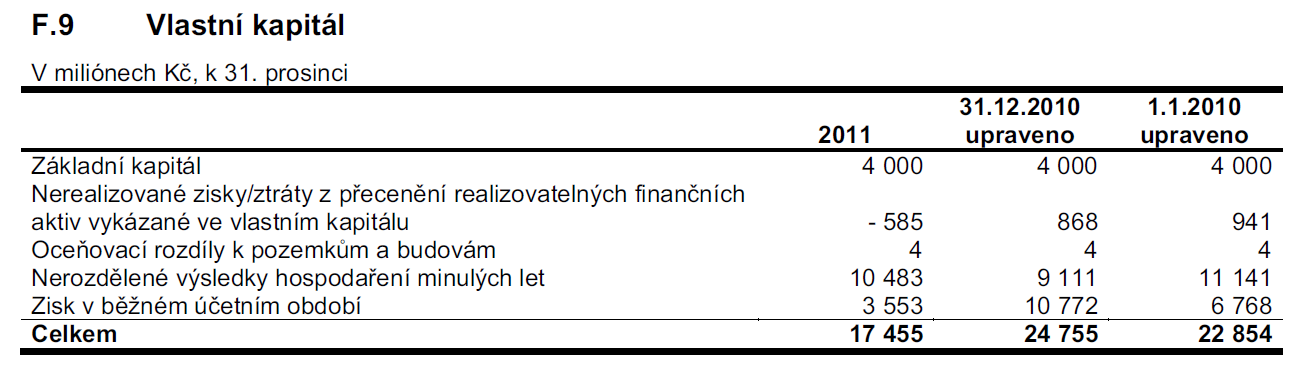
\includegraphics[width=1.0\textwidth]{cp-vlk.png}
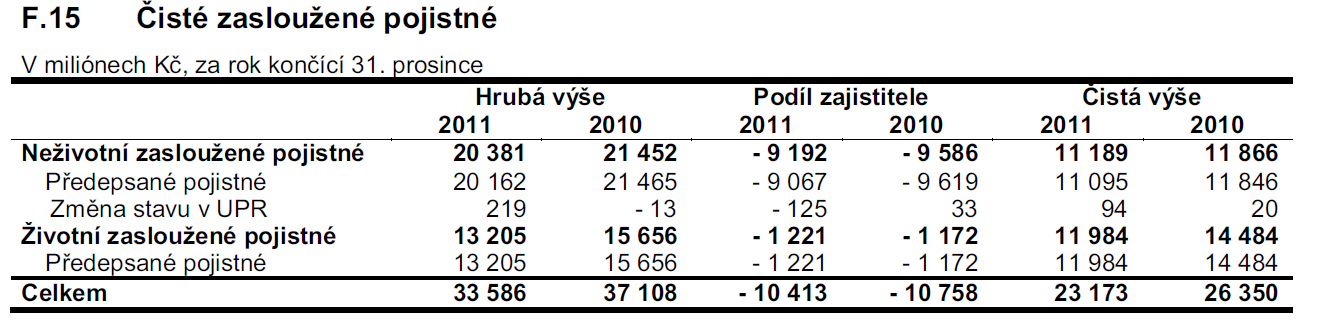
\includegraphics[width=1.0\textwidth]{cp-poj.png}
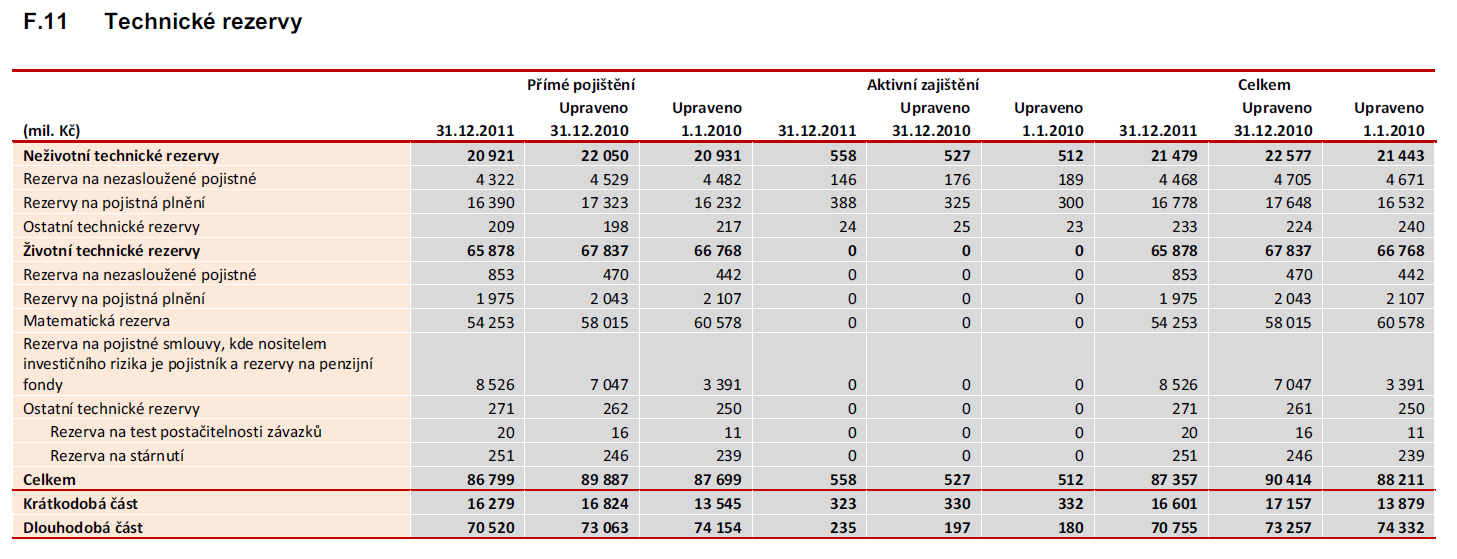
\includegraphics[width=1.0\textwidth]{cp-tr.png}
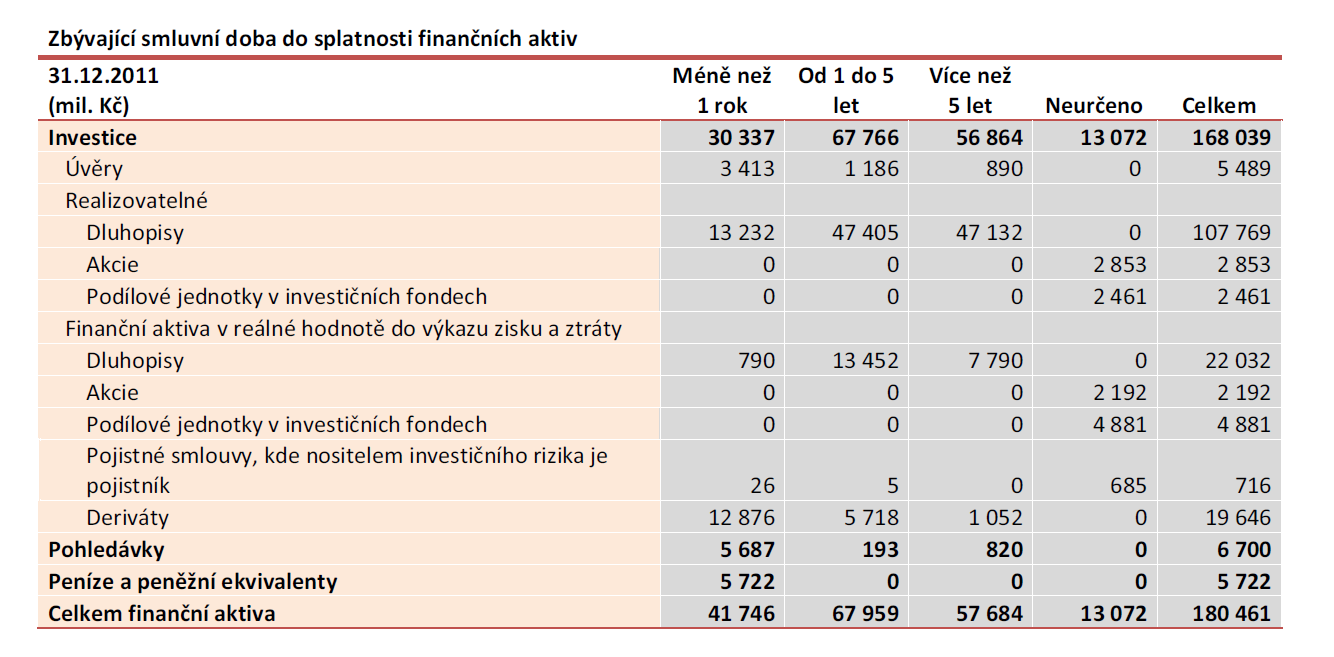
\includegraphics[width=1.0\textwidth]{cp-likv.png}
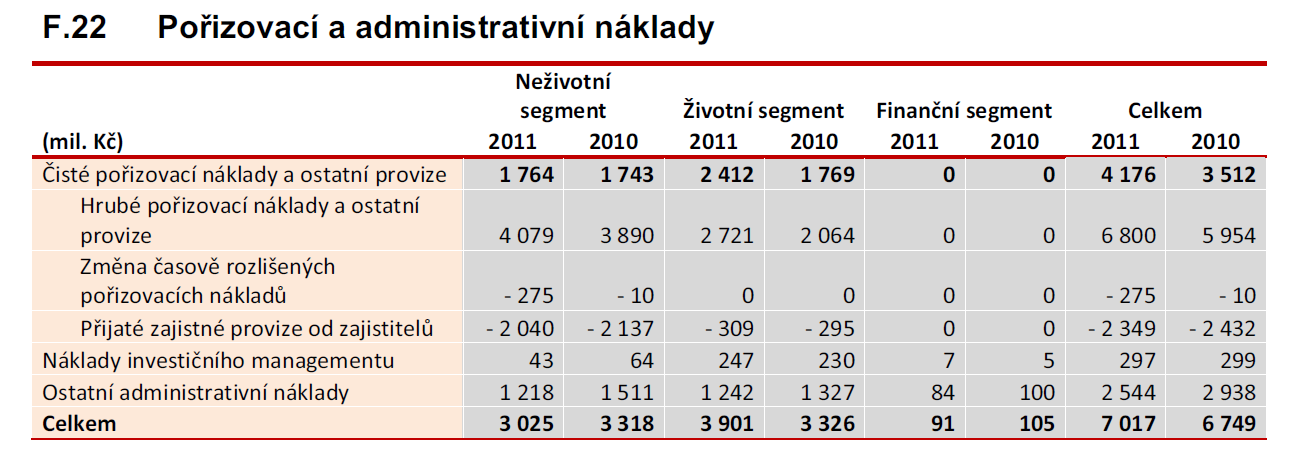
\includegraphics[width=1.0\textwidth]{cp-nakl.png}
\begin{align*}
	\text{solvency ratio}&=\frac{17 455-4 000}{23 173}=0.5806\\
	\text{ukazatel TR}&=\frac{87 357+17 455}{23 173}=4.5230\\
	\text{ukazatel TR NŽP}&=\frac{21479+17 455\cdot\frac{11189}{23173}}{11189}=2.6729\\
	\text{ukazatel TR ŽP}&=\frac{65876+17 455\cdot\frac{11984}{23173}}{11984}=6.2502\\
	\text{retention ratio}&=\frac{33586-4176}{33 586}=0.8756\\
	\text{liquidity ratio}&=\frac{41 764}{87 357}=0.4778\\
	\text{expenses ratio}&=\frac{7 017}{33 586}=0.2089\\
\end{align*}
\section{Allianz}
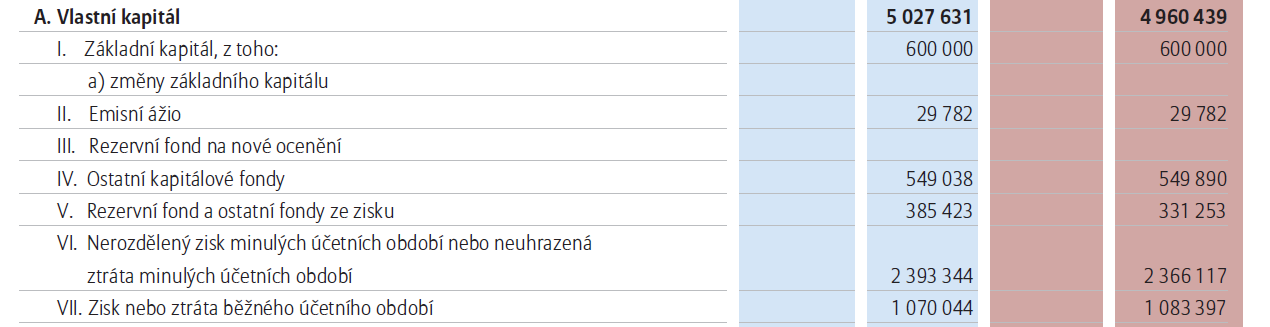
\includegraphics[width=1.0\textwidth]{al-vlk.png}
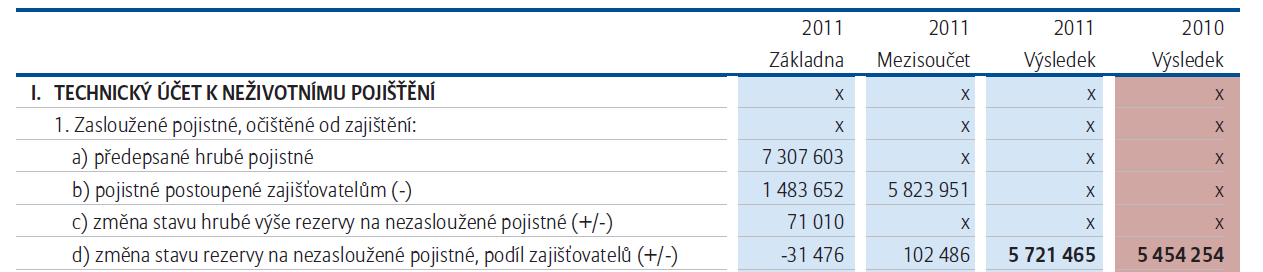
\includegraphics[width=1.0\textwidth]{al-poj1.png}
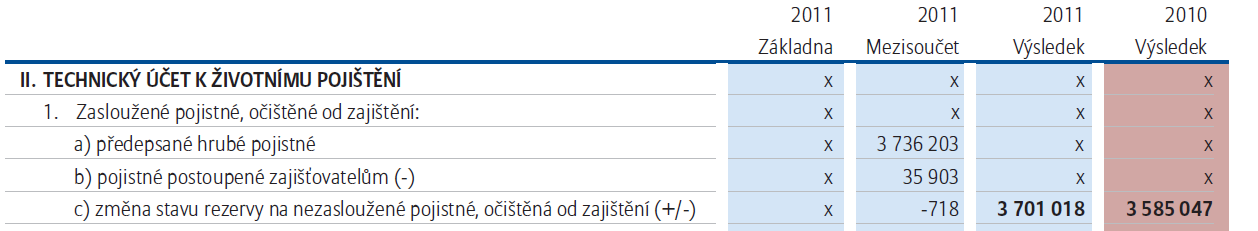
\includegraphics[width=1.0\textwidth]{al-poj2.png}

\includegraphics[width=1.0\textwidth]{al-tr.png}
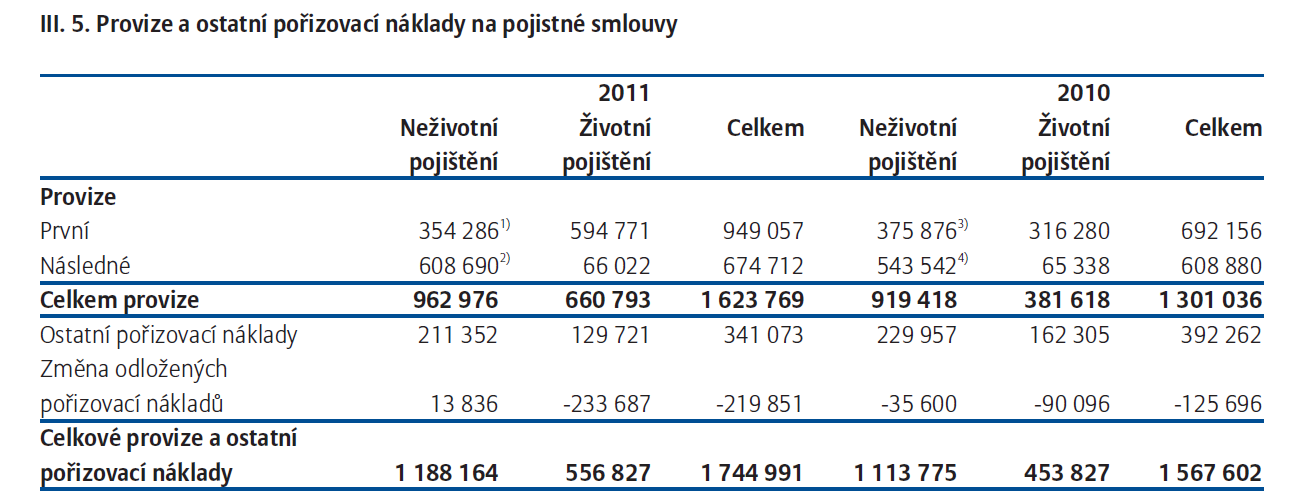
\includegraphics[width=1.0\textwidth]{al-nakl1.png}
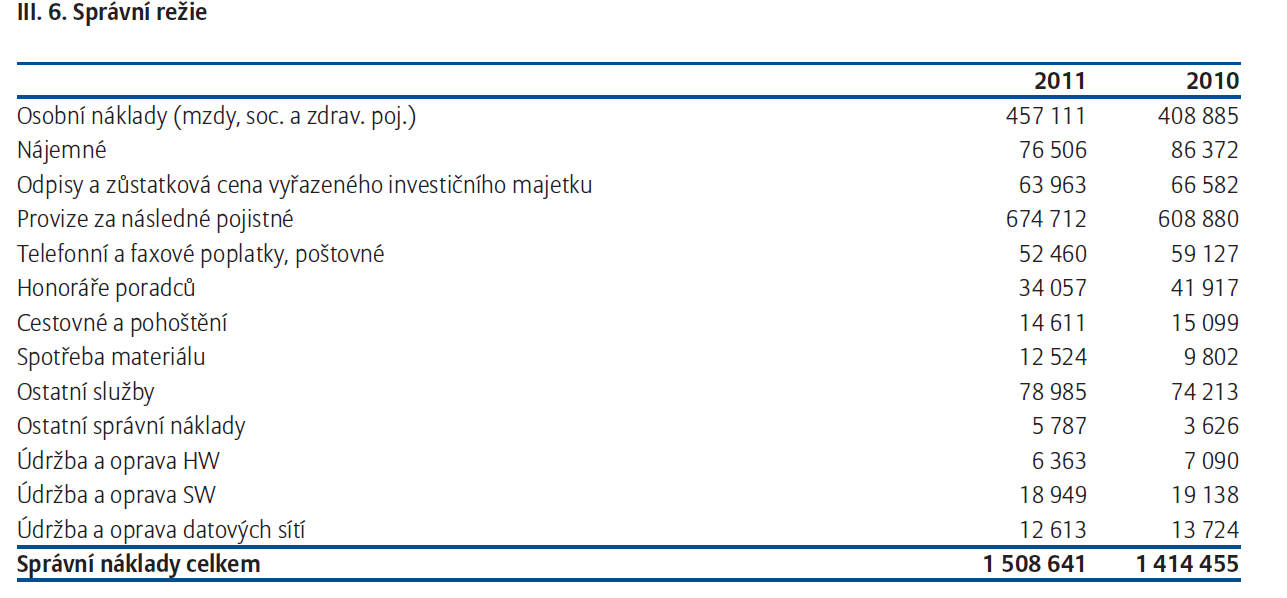
\includegraphics[width=1.0\textwidth]{al-nakl2.png}
\begin{align*}
	\text{čisté pojistné}&=5827+3701=9524\\
	\text{solvency ratio}&=\frac{5027-600}{9524}=0.4648\\
	\text{ukazatel TR}&=\frac{14322+5027}{9524}=2.0316\\
	\text{retention ratio}&=\frac{11044-1576}{11044}=0.8581\\
	\text{expenses ratio}&=\frac{1744+1508}{11044}=0.2944\\
\end{align*}
\section{Závěr}
Ukazatel solventnosti obou zkoumaných pojišťoven je významně nad 30\%, což je doporučovaná spodní hranice. Výše technických rezerv je několikanásobkem čistého pojistného. Při rozdělení na životní a neživotní složku vidíme, že u životního pojištění u České pojišťovny dosahuje tento násobek více než 6. To lze vysvětlit tím, že mnoho smluv životního pojištění ješte nebylo vyplaceno, kvůli tomu, že český pojišťovací sektor je poměrně mladý. Lze předpokládat, že na vyspělejších trzích tomu tak nebude. Nákladovost dosahuje 20 až 30 \%. Ze sledovaných ukazatelů lze říci, že Česká pojišťovna je solventnější než Allianz pojišťovna.
\end{document}